\documentclass[12pt]{article}
% ----------------------------------------------------------------------
% Define external packages, language, margins, fonts, new commands 
% and colors
% ----------------------------------------------------------------------
\usepackage[utf8]{inputenc} % Codification
\usepackage[english]{babel} % Writing idiom

\usepackage[export]{adjustbox} % Align images
\usepackage{amsmath} %a Extra commands for math mode
\usepackage{amssymb} % Mathematical symbols
\usepackage{anysize} % Personalize margins
    \marginsize{2cm}{2cm}{2cm}{2cm} % {left}{right}{above}{below}
\usepackage{appendix} % Appendices
\usepackage{cancel} % Expression cancellation
\usepackage{caption} % Captions
    \captionsetup{labelfont={bf}}
\usepackage{cite} % Citations, like [1 - 3]
\usepackage{color} % Text coloring
\usepackage{fancyhdr} % Head note and footnote
    \pagestyle{fancy}
    \fancyhf{}
    \fancyhead[L]{
        
\includegraphics[scale = 0.3]{Images/NovaFctHor.png}
    } % Left of Head note
    \fancyhead[R]{\footnotesize SDc} % Right of Head note
    \fancyfoot[L]{\footnotesize MEEC} % Left of Footnote
    \fancyfoot[R]{\thepage  } % Center of Footnote
    %\fancyfoot[R]{\footnotesize Degree} % Right of Footnote
    \renewcommand{\footrulewidth}{0.4pt} % Footnote rule
\usepackage{float} % Utilization of [H] in figures
\usepackage{graphicx} % Figures in LaTeX
\usepackage[colorlinks = true, plainpages = true, linkcolor = novablue, urlcolor = novablue, citecolor = novablue, anchorcolor = novablue]{hyperref}
\usepackage{indentfirst} % First paragraph
\usepackage[super]{nth} % Superscripts
\usepackage{siunitx} % SI units
\usepackage{subcaption} % Subfigures
\usepackage{titlesec} % Font
    \titleformat{\section}{\Large\bfseries}{\thesection}{1em}{}
    \titleformat{\subsection}{\large\bfseries}{\thesubsection}{1em}{}
    \titleformat{\subsubsection}{\normalsize\bfseries}{\thesubsubsection}{1em}{}
    %\fancyfoot[C]{\thepage}

%code
\usepackage[breakable]{tcolorbox}

% Code highlighting
\usepackage{listings}
\lstset{ 
    backgroundcolor=\color{cellbackground}, % background color for the code block
    basicstyle=\ttfamily,                   % font style
    breakatwhitespace=false,                % automatic breaks only at whitespace
    breaklines=true,                        % automatic line breaking
    captionpos=b,                           % caption position
    commentstyle=\color{gray},              % comment style
    escapeinside={\%*}{*)},                 % if you want to add LaTeX within your code
    keywordstyle=\color{blue},              % keyword style
    stringstyle=\color{dkgreen},            % string style
    frame=single,                           % adds a frame around the code
    rulecolor=\color{cellborder},           % border color
}

%---------TIKZ CONFIG---------%
%Block diagram
\usepackage{tikz}
\usetikzlibrary{positioning, shapes.geometric, arrows}
% Define custom color lightblue
\definecolor{lightblue}{RGB}{173, 216, 230}
\tikzstyle{block} = [draw, rectangle, 
    minimum height=2.5em, minimum width=3.5em]
\tikzstyle{arrow} = [thick,->,>=stealth]
\tikzstyle{sum} = [draw, circle, node distance=1cm, minimum width=2em]
\tikzstyle{input} = [coordinate]
\tikzstyle{pinstyle} = [pin edge={to-,thin,black}]
%---------TIKZ CONFIG---------%

% Exact colors from NB
\definecolor{incolor}{HTML}{303F9F}
\definecolor{outcolor}{HTML}{D84315}
\definecolor{cellborder}{HTML}{CFCFCF}
\definecolor{cellbackground}{HTML}{F7F7F7}

%folders .tex
\usepackage{subfiles}

% Random text (not needed)
\usepackage{lipsum}
\usepackage{duckuments}

% Tables
\usepackage{tabularx} 
\usepackage{booktabs}
\usepackage{makecell}

% New and re-newcommands
\newcommand{\sen}{\operatorname{\sen}} % Sine function definition
\newcommand{\HRule}{\rule{\linewidth}{0.5mm}} % Specific rule definition
\renewcommand{\appendixpagename}{\LARGE Appendices}

% Colors

\definecolor{novablue}{RGB}{0, 101, 189}
\definecolor{dkgreen}{RGB}{52,129,65}

%%%%%%%%%%%%%%%%%%%%%%%%%%%%%%%%%%%%%%%%%%%%%%%%%%%%%%%%%%%%%%%%%%%%%%%%
%                                 Document                             %
%%%%%%%%%%%%%%%%%%%%%%%%%%%%%%%%%%%%%%%%%%%%%%%%%%%%%%%%%%%%%%%%%%%%%%%%
\begin{document}
% Add bibliography data and style
\bibliographystyle{IEEEtran}
% ----------------------------------------------------------------------
% Cover
% ----------------------------------------------------------------------
\begin{center}
    \begin{figure}
        \vspace{-1.0cm}
        
\includegraphics[scale = 0.055, left]{Images/NovaFctVer.png} % Nova logo
        
    \end{figure}

    \mbox{}\\[2.0cm]
    \textsc{\Huge Mestrado em Engenharia Eletrotécnica e de Computadores}\\[2.5cm]
    \textsc{\LARGE Sistemas de Decisão}\\[2.0cm]
    \HRule\\[0.4cm]
    {\large \bf {Final Project}}\\[0.2cm]
    \HRule\\[1.5cm]
\end{center}

\begin{flushleft}
    \textbf{Author:}
\end{flushleft}

\begin{center}
    Filipe Cavalheiro
\end{center}
 
% Caixa a dizer o grupo
%\begin{flushleft}
%    \large $\boxed{\text{\bf Group} \ \clubsuit}$\\[4.0cm]
%\end{flushleft}

\vspace{5cm}

\begin{center}
    \large \bf 2024/2025 -- \nth{2} Semester, DEEC
\end{center}

\thispagestyle{empty}

\setcounter{page}{0}

\newpage

\newpage

\tableofcontents % Generates the table of contents

\newpage

\listoffigures

\newpage

\section{Introduction}
In this project it was defined to create a decision system ca'able of maneuvering a ground vehicle 
that has fault detection and collision avoidance.\\

A total of 3 iterations making os that the report is split in the following sections, I linear system, II non linear system,
III Optimized system, IV Future Improvements, V Conclusions.\\

\section{Linear System (1st Iteration)}
For an easier first implementation of the problem a linear system was consider being the state space variable, position and velocity.
Having an actuation in acceleration of the vehicle.

\subsection{State Space}
The consider state space was a double integrator.

The A matrix as follows:

\begin{equation*}
    A = 
    \begin{bmatrix}
     1& 0& dt& 0\\
     0& 1& 0& dt\\
     0& 0& 1& 0\\
     0& 0& 0& 1\\
    \end{bmatrix}
\end{equation*}

Our B matrix as: 

\begin{equation*}
    B = 
    \begin{bmatrix}
    \frac{1}{2} dt^2 & 0\\
    0& \frac{1}{2} dt^2\\
    dt& 0\\
    0& dt\\
    \end{bmatrix}
\end{equation*}

\subsection{System architecture}

To facilitate the understanding of the following subsections, the complete system architecture is presented 
in Figs~\ref{fig:Main_system_architecture},\ref{fig:Fault_Detection_System}. 
This architecture illustrates the main components of the system and how they interact, including the reference 
generation, path planning, observer-based fault detection, and navigation control modules.

\begin{figure}[H]
    \centering
    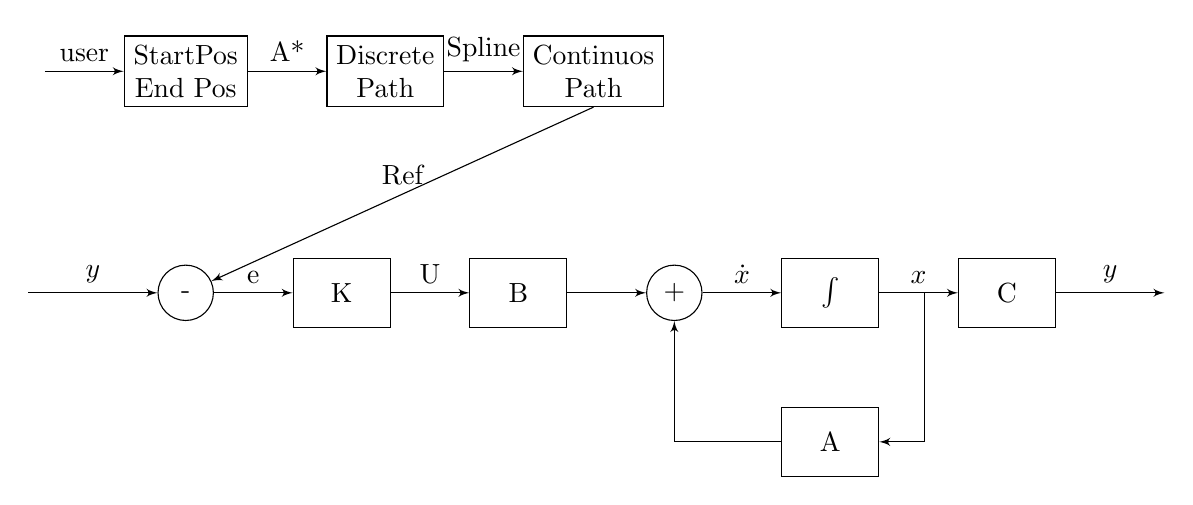
\begin{tikzpicture}[auto, node distance=1cm,>=latex']
        % We start by placing the blocks
        \node [input, name=input] {};
        \node [block, align=center, right  =of input] (StartPos) {StartPos\\End Pos};
        \node [block, align=center, right  =of StartPos] (Discrete_Path) {Discrete\\Path};
        \node [block, align=center, right =of Discrete_Path] (Continuos_Path) {Continuos\\Path};
        \node [sum, align=center, below =2cm of StartPos] (sum_1) {-};
        \node [block, align=center, right =of sum_1] (Gain) {K};
        \node [block, align=center, right  =of Gain] (B) {B};
        \node [sum, align=center, right =of B] (sum_2) {+};
        \node [block, align=center, right =of sum_2] (Integrator) {$\int$};
        \node [block, align=center, right =of Integrator] (C) {C};
        \node [block, align=center, below =of Integrator] (A) {A};

        \draw[->] (input) -- (StartPos) node[midway, above]{user};
        \draw[->] (StartPos) -- (Discrete_Path) node[midway, above]{A*};
        \draw[->] (Discrete_Path) -- (Continuos_Path) node[midway, above]{Spline};
        \draw[->] (Continuos_Path.south) -- (sum_1) node[midway, above]{Ref};
        \draw[->] (sum_1) -- (Gain) node[midway, above]{e};
        \draw[->] (Gain) -- (B) node[midway, above]{U};
        \draw[->] (B) -- (sum_2);
        \draw[->] (sum_2) -- (Integrator) node[midway, above]{$\dot{x}$};
        \draw[->] (Integrator) -- (C) node[midway, above]{$x$};
        \draw[->] (C) -- ++(2,0) node[midway, above]{$y$};
        \draw[->] (Integrator)++(1.2,0) |- (A);
        \draw[->] (A) -| (sum_2);
        \draw[->] (sum_1)++(-2,0) -- (sum_1) node[midway, above]{$y$};
    \end{tikzpicture}
    \caption{Main system architecture}
    \label{fig:Main_system_architecture}
\end{figure}

\begin{figure}[h]
    \centering
    \begin{tikzpicture}[auto, node distance=1cm,>=latex']
        % Observer group, 10cm below everything else
        \node [input, name=input] {};
        \node [block, align=center, right=of input] (Obs_B) {B};
        \node [sum, align=center, right=of Obs_B] (Obs_sum2) {+};
        \node [block, align=center, right=of Obs_sum2] (Obs_Integrator) {$\int$};
        \node [sum, align=center, right=of Obs_Integrator] (Obs_sum3) {+};
        \node [sum, minimum size=0.25cm] (ye) at (Obs_sum3.center) {};
        \node [block, align=center, right=of Obs_sum3] (Obs_C) {C};
        \node [block, align=center, below=of Obs_Integrator] (Obs_A) {A};
        \node [sum, align=center, right=of Obs_C] (intersect) {$\cap$};
        \node [sum, align=center, above=of intersect] (Obs_sum4) {+};
        \node [sum, minimum size=0.25cm] (ye) at (Obs_sum4.center) {};

        \draw[->] (Obs_B)++(-2,0) -- (Obs_B) node[midway, above]{U};
        \draw[->] (Obs_sum2) -- (Obs_Integrator) node[midway, above]{$\dot{X}$};
        \draw[->] (Obs_Integrator) -- (Obs_sum3) node[midway, above]{$X$};
        \draw[->] (Obs_sum3) -- ++(Obs_C);
        \draw[->] (Obs_Integrator)++(1.2,0) |- (Obs_A);
        \draw[->] (Obs_B) -- (Obs_sum2);
        \draw[->] (Obs_C) -- (intersect) node[midway, above]{$Y$};
        \draw[->] (Obs_A) -| (Obs_sum2);
        \draw[->] (Obs_sum3)++(0, -1) node[below]{$W$} -- (Obs_sum3);
        \draw[->] (Obs_sum4) -- (intersect);
        \draw[->] (Obs_sum4)++(-1,0) node[left]{$V$} -- (Obs_sum4);
        \draw[->] (Obs_sum4)++(1,0) node[right]{$y$} -- (Obs_sum4);
        \draw[->] (intersect) -- ++(1,0) node[right]{Fault Detection} (intersect) ;
    \end{tikzpicture}
    \caption{Fault Detection System}
    \label{fig:Fault_Detection_System}
\end{figure}

\subsection{Obtaining a Reference}

As shown in the system architecture, the reference trajectory is obtained by generating a path from the vehicle's 
initial position to a desired final position.\\

The path is planned using the A* algorithm, a discrete graph-based method for path finding capable of accounting for 
obstacles that may exist between the start and end positions.\\

However, since A* produces a discrete sequence of waypoints and the vehicle requires a continuous and smooth trajectory 
to follow, a third-order polynomial is fitted between consecutive waypoints to interpolate the path.\\

It is important to note that the path is computed only once at the beginning of the operation. During the vehicle's 
movement, obstacles may change in size or position, which makes this static planning approach valid but insufficient 
for guaranteeing safe and collision-free navigation throughout the mission. This limitation is addressed later in Section 
\ref{sec:System Optimization (3rd Implementation)}.\\

Additionally, while algorithms such as D* offer more efficient dynamic replanning by updating only the necessary 
portions of the path, this optimization was not implemented due to time constraints. Nonetheless, this omission 
does not compromise the fulfillment of the main project requirements.

\subsection{Control system}
A simple state feedback gain control system was implemented, with the controller designed by placing four poles, 
one for each system state.

\begin{equation*}
    \begin{bmatrix}
        0.2& 0.3& 0.5& 0.4
    \end{bmatrix}
\end{equation*}

Due to time constraints and since advanced control design was not the primary focus of this project, 
this approach was considered sufficient to meet the system requirements. However, alternative control 
strategies such as PID controllers or Model Predictive Control (MPC) could have been explored and 
implemented in future work.

\subsection{Fault Detection}
A deterministic observer was implemented to ensure safe navigation by detecting potential obstacles and system faults. 
This observer operates as a parallel copy of the real system, receiving the same control inputs. 
It predicts the expected system state and output within a defined uncertainty region — represented as a square in the state 
and output space.\\

At each time step, the actual system output is compared against this predicted uncertainty region. 
If the real system state falls outside this region, it is flagged as a fault condition.\\

For navigation safety, the state variances in the x and y positions are computed at each step. 
These variances are used to dynamically adjust the size of obstacles within the path planning algorithm, 
causing them to expand or contract as necessary. The path planner is expected to modify the planned route 
accordingly to maintain the shortest and safest trajectory to the target destination. However, in this iteration, 
an unresolved bug prevents the path from updating in response to these obstacle changes. This 
issue has been addressed in subsequent versions of the system.\\

The disturbance and noise sets have not been chosen in a deterministic process but were instead estimated heuristically. 
This comes to my poor understanding of how to choose this sets, time constraints and honestly just work exhaustion. 
(not this work but in general)\\

It is acknowledged that a more rigorous approach would involve analyzing experimental 
data collected from the system under nominal conditions, alongside the desired path, to compute 
the variance of the observed values. This would enable a clearer separation between variance 
contributions from sensor noise and from external disturbances. However, without this analysis,
the precise attribution of variance sources remains uncertain.\\

Future work should address this limitation by experimentally characterizing the system's noise and 
disturbance profiles to improve the accuracy and reliability of the observer and fault detection scheme.

\section{Non linear system (Second implementation)}

For this implementation the original dual integrator system has been replaced with a non linear system.
This system's state space is controlled via force and torque. Being the the state defined by the vehicle's position,
angle, velocity and angular velocity.

\begin{equation*}
    \begin{bmatrix}
        X_{pos}&Y_{pos}&\theta&v&\omega
    \end{bmatrix}
\end{equation*}

\subsection{Feedback Linearization}
We can write the dynamics with respect to a point with distance $L$ from the center of mass  

\[
h_x = p_x + L \cos(\theta)
\]
\[
h_y = p_y + L \sin(\theta)
\]

Taking the second derivative it becomes 

\[
\begin{bmatrix}
    \ddot{h}_x \\
    \ddot{h}_y
\end{bmatrix}
=
\underbrace{
\begin{bmatrix}
    \cos(\theta) & -\sin(\theta) \\
    \sin(\theta) & \cos(\theta)
\end{bmatrix}
}_{\mathbf{R}(\theta)}
\begin{bmatrix}
    F/m - L w^2 \\
    TL/J + v w
\end{bmatrix}
\]

And if we use the control law  

\[
\begin{bmatrix}
F \\
T
\end{bmatrix}
=
\begin{bmatrix}
m & 0 \\
0 & J/L
\end{bmatrix}
\left(
\mathbf{R}(-\theta)
\begin{bmatrix}
u_x \\
u_y
\end{bmatrix}
-
\begin{bmatrix}
- L w^2 \\
v w
\end{bmatrix}
\right)
\]

The dynamics becomes  

\[
\ddot{h}_x = u_x
\]
\[
\ddot{h}_y = u_y
\]

Making so that we can use a double integrator once again as in the original system.
Since we have direct access to the position and velocity of the vehicle this state values are passed to the linear state space
which converts them to control actuation for the non linear state space.

\section{System Optimization (3rd Implementation)} \label{sec:System Optimization (3rd Implementation)}

Several optimizations were introduced in this third implementation of the system. The most significant improvement was 
the recalculation of the trajectory at every time step, taking into account the updated dimensions of the obstacles. 
Additionally, obstacles that were previously modeled as circles were reformulated as ellipses, allowing the system to 
account for the vehicle's position variance independently in the x and y directions and expand or 
contract the objects accordingly.\\

\section{Results and Conclusions}

The final result obtained has achieved the desired goal of navigation with collision avoidance.
The following Fig.~\ref{fig:results} shows the achieved path contouring a circle while maintaining a safe distance from the same. 
it is recommended to run the code in order to see the evolution of the path as well as the object shrinkage and expansion.
Despite some possible improvements being mentioned below~\ref{sec:Improvements and Known Errors} it was consider that the 
result is satisfactory for the desired purposes.

\begin{figure}[h]
    \centering
    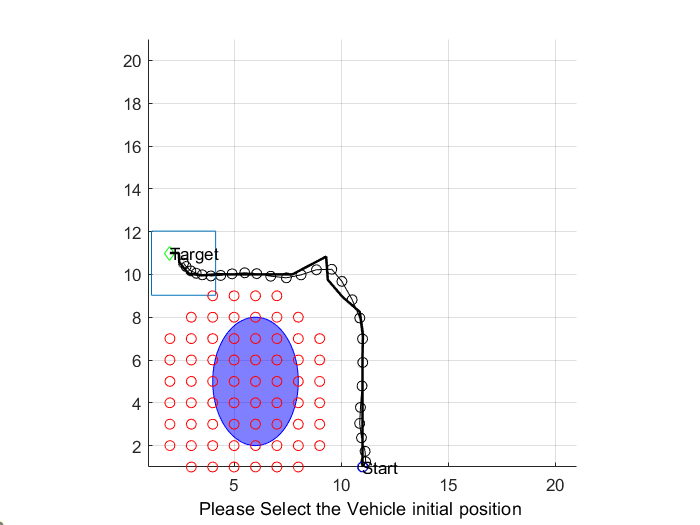
\includegraphics[width=16cm]{Images/results.png}
    \caption{Vehicle trajectory results}
    \label{fig:results}
\end{figure}

The developed system successfully achieved its main goal of autonomous navigation with collision avoidance. 
Through three implementations — starting from a linear model, evolving to a nonlinear system with feedback linearization, 
and finally introducing dynamic path replanning — the project progressively improved both safety and performance.\\

While several limitations remain, including heuristic observer tuning and the absence of real experimental data, 
the final system reliably detects obstacles and adjusts its path accordingly. The modular structure also leaves room 
for future enhancements, such as integrating dynamic planning algorithms like D* and refining control strategies.\\

Overall, the results are satisfactory for the intended objectives and establish a solid base for future improvements.

\section{Unused implementation}
At one stage of development, it was mistakenly assumed that the nonlinear system would not have direct access to the vehicle's 
speed measurement. As a result, a Kalman filter was implemented to estimate this state. However, after realizing that the 
speed was directly available, this implementation became unnecessary. The Kalman filter code remains in the project files 
but is not used in the final implementation.

\section{Improvements and Known Errors} \label{sec:Improvements and Known Errors}

As previously mentioned, several improvements could be made to enhance the system's performance, robustness, and efficiency. 
Additionally, some limitations and known issues were identified during development. These are summarized below:

\begin{itemize}
    \item Path Planning Efficiency:
The current implementation recalculates the entire path at every time step, which is computationally inefficient. 
A more appropriate approach would be to use a dynamic path planning algorithm such as D* or D*-Lite, which incrementally 
updates only the affected portions of the path as new obstacle information becomes available. Since only the immediate 
next actuation is typically of interest, this would significantly reduce computational load.
    \item Simplistic Control Law:
The control system was implemented using a simple state feedback gain with pole placement. While sufficient for the 
project's requirements, more advanced control strategies such as PID controllers, LQR, or Model Predictive Control 
(MPC) could offer better performance, particularly in terms of trajectory tracking and disturbance rejection.
    \item Absence of Real Experimental Data:
Despite being one of the original project requirements, real experimental data was not incorporated into the 
system due to time constraints and workload exhaustion. This omission prevented the validation of observer 
performance, disturbance modeling, and fault detection reliability against actual system behavior.
    \item Reference Tracking Issues:
The reference tracking implementation is fundamentally flawed. The system assumes that the vehicle moves 
along the planned path at a constant rate, without considering its actual position. Specifically, the system 
defines 300 evenly spaced points between the start and end positions and advances to the next reference point 
at every time step, effectively operating in open loop. This results in significant tracking errors, as the 
reference point may not correspond to the vehicle's current location.
    \item Observer Tuning by Heuristics:
The disturbance and noise uncertainty bounds in the deterministic observer were chosen heuristically rather 
than determined through a systematic, data-driven process. As a result, fault detection performance may be 
either too conservative or insufficiently sensitive, depending on operating conditions.
    \item Grid Resolution Constraints:
The A* algorithm was implemented on a discrete grid using natural numbers. This restricts the resolution of 
the path, especially in narrow passages or cluttered environments. Furthermore, when updating the starting 
position for path recalculation, the vehicle's continuous position is approximated to the nearest grid point, 
introducing an additional source of tracking error.
    \item Lack of Closed-Loop Reference Updating:
No feedback-based mechanism was used to adjust the reference point based on the actual vehicle position. 
A closed-loop reference tracking system, which selects the nearest point on the planned path relative to the current 
vehicle position, would help mitigate cumulative tracking errors.
    \item   No System Identification Performed:
The vehicle's dynamic model was assumed to be perfectly known and constant. In practical scenarios, 
discrepancies between the modeled and actual system dynamics can degrade both control performance and observer accuracy. 
Incorporating system identification techniques would improve model fidelity and system reliability.
\end{itemize}

\section{Appendix}

\subsection{First Iteration}\label{anex:First Iteration}
\begin{lstlisting}
   close all;
clearvars;
addpath(genpath('YALMIP-develop'))   % YALMIP, https://github.com/yalmip/YALMIP
addpath(genpath('ReachTool-main'))   % ReachTool (constrained zonotopes), provided in the course
addpath(genpath('Astar'))

%variabels
r = 2;
center = [6,4];
vehicle_mass = 500;    % grams
vehicle_fuel = 500;    % grams
fuel_rate = 10;        % grams per step

cycles_with_fuel = vehicle_fuel / fuel_rate;
extra_steps = 0;     % Steps after fuel ends
total_steps = cycles_with_fuel + extra_steps;
dt = 1;

%circle definition
th = 0:pi/50:2*pi;
x_obj = r * cos(th) + center(1);
y_obj = r * sin(th) + center(2);
% Vector from centroid to each point
dx = x_obj - center(1);
dy = y_obj - center(2);
lengths = r/2;
dx_unit = dx ./ lengths;
dy_unit = dy ./ lengths;

% State-space matrices
A = [1 0 dt 0;
     0 1 0 dt;
     0 0 1 0;
     0 0 0 1];
B = [0.5*dt^2 0;
    0 0.5*dt^2;
    dt 0;
    0 dt]; 
C = kron([1,0],eye(2));

% draw the trajectory of the vehicle
figure;
hold on;
axis equal; grid on;
fill(x_obj, y_obj, 'b', 'FaceAlpha', 0.5, 'EdgeColor', 'b'); %object
drone = animatedline('Marker','o');
estimate = plot(1,1);
detected = false;

maximum_variance = 0.1;
real_xsim = zeros(1, total_steps);
real_ysim = zeros(1, total_steps);

%DEFINE THE 2-D MAP ARRAY
MAX_X=20;
MAX_Y=20;
%This array stores the coordinates of the map and the 
%Objects in each coordinate
MAP=2*(ones(MAX_X,MAX_Y));

points = integer_points_in_circle(center, r+maximum_variance, r+maximum_variance);
MAP(points(:, 1),points(:,2)) = -1; %add new circle
plot(points(:, 1)+0.5, points(:,2)+0.5,'ro');

% Obtain Obstacle, Target and Robot Position
% Initialize the MAP with input values
% Obstacle=-1,Target = 0,Robot=1,Space=2
j=0;
x_val = 1;
y_val = 1;
axis([1 MAX_X+1 1 MAX_Y+1])
grid on;
hold on;
n=0;%Number of Obstacles

% BEGIN Interactive Obstacle, Target, Start Location selection
xlabel('Please Select the Target using the Left Mouse button','Color','black');
but=0;
while (but ~= 1) %Repeat until the Left button is not clicked
    [xval,yval,but]=ginput(1);
end
xval=floor(xval);
yval=floor(yval);
xTarget=xval;%X Coordinate of the Target
yTarget=yval;%Y Coordinate of the Target

MAP(xval,yval)=0;%Initialize MAP with location of the target
plot(xval+.5,yval+.5,'gd');
text(xval+1,yval+.5,'Target')

xlabel('Select Obstacles using the Left Mouse button,to select the last obstacle use the Right button','Color','blue');
while but == 1
    [xval,yval,but] = ginput(1);
    xval=floor(xval);
    yval=floor(yval);
    MAP(xval,yval)=-1;%Put on the closed list as well
    plot(xval+.5,yval+.5,'ro');
end%End of While loop

xlabel('Please Select the Vehicle initial position ','Color','black');
but=0;
while (but ~= 1) %Repeat until the Left button is not clicked
    [xval,yval,but]=ginput(1);
    xval=floor(xval);
    yval=floor(yval);
end

xStart=xval;%Starting Position
yStart=yval;%Starting Position
MAP(xval,yval)=1;
plot(xval+.5,yval+.5,'bo');
text(xval+1,yval+.5,'Start')
%End of obstacle-Target pickup

% State vector: [x; y; vx; vy]
state = zeros(4, total_steps + 1);
state(1:2,1) = [xStart;yStart];  % Initial position
y = zeros(2, total_steps + 2);

% Define a feedback controller
K = place(A,B,[0.5 0.2 0.4 0.3]);

[m,n] = size(C); % dimensions of output and state

% Observers - 1: Nominal model
X = cell(1, total_steps); 
X{1}.G = diag([xStart, yStart, 0, 0]);
X{1}.c = zeros(n,1);
X{1}.A = zeros(0,n);
X{1}.b = zeros(0,1);

% disturbance set
W.G = 1.25*eye(n);
W.c = zeros(n,1);
W.A = zeros(0,n);
W.b = zeros(0,1);

% noise set
V.G = 1.5*eye(2);
V.c = zeros(2,1);
V.A = zeros(0,2);
V.b = zeros(0,1);

% Loop through each time step
for k = 1:total_steps
    MAP(points(:, 1),points(:,2)) = 1; %remove last circle
    
    points = integer_points_in_circle(center, r + maximum_variance, r+maximum_variance);
    points = max(points,1);
    MAP(points(:, 1),points(:,2)) = -1; %add new circle
    plot(points(:, 1)+0.5, points(:,2)+0.5,'ro');
    Optimal_path = Astar(MAX_X, MAX_Y, MAP,xval, yval, xTarget, yTarget, xStart, yStart);

    % j=size(Optimal_path,1);
    % %Plot the Optimal Path!
    % plot(Optimal_path(:,1)+.5,Optimal_path(:,2)+.5);
    x_trajectory = flip(Optimal_path(:,1)');
    y_trajectory = flip(Optimal_path(:,2)');
    % Move points outward
    % x_trajectory = x_obj + dx_unit*maximum_variance;
    % y_trajectory = y_obj + dy_unit*maximum_variance;
    
    % Parametric t values based on cumulative distance
    distances = sqrt(diff(x_trajectory).^2 + diff(y_trajectory).^2);
    t_points = [0, cumsum(distances)];
    
    % Compute spline coefficients for x(t) and y(t)
    coeffs_x = computeSplineCoefficients(t_points, x_trajectory);
    coeffs_y = computeSplineCoefficients(t_points, y_trajectory);
    
    % Evaluate splines at fine t grid
    tsim = linspace(t_points(1), t_points(end), total_steps);
    xsim = zeros(size(tsim));
    ysim = zeros(size(tsim));
    
    % Evaluate each interval
    for i = 1: length(t_points)-1
        idx = tsim >= t_points(i) & tsim <= t_points(i+1);
        dt = tsim(idx) - t_points(i);
    
        c_x = coeffs_x((i-1)*4 + (1:4));
        xsim(idx) = polyval([c_x(4) c_x(3) c_x(2) c_x(1)], dt);
    
        c_y = coeffs_y((i-1)*4 + (1:4));
        ysim(idx) = polyval([c_y(4) c_y(3) c_y(2) c_y(1)], dt);
    end
    real_xsim(k) = xsim(k);
    real_ysim(k) = ysim(k);
    ref = [xsim; ysim; zeros(size(tsim)); zeros(size(tsim))];
    
    if k == 1
        path_line = plot([real_xsim(1:k) xsim(k+1:end)], [real_ysim(1:k) ysim(k+1:end)], 'k-', 'LineWidth', 1.5);
    else
        set(path_line, 'XData', [real_xsim(1:k) xsim(k+1:end)], 'YData', [real_ysim(1:k) ysim(k+1:end)]);
    end

    if k <= cycles_with_fuel
        u = -K*(state(:,k)-ref(:,k)); % controller
    else
        u = [0; 0];  % No acceleration after fuel runs out
    end
    state(:,k+1) = A * state(:,k) + B *u;
    y(:,k+1) = C*state(:,k+1);

    % Run the observer
    X{k+1} = CZMinkowskiSum(CZLinMap(A,X{k},B*u),W);
    Y = CZLinMap(-eye(2),V,y(:,k));
    X{k} = CZIntersect(C,X{k},Y);

    [F,p] = compileCZ(X{k});

    setPoints = plot(F,p(1:2));

    if size(setPoints{1},2)==1 && ~detected
        fprintf("There is a fault at the iteration k = %d\n",k);
        detected = true;
    end

    % update the set-valued estimate
    set(estimate,'Xdata',setPoints{1}(1,:),'Ydata',setPoints{1}(2,:));
    x_variance_length = (max(setPoints{1}(1,:))-min(setPoints{1}(1,:)))/2;
    y_variance_length = (max(setPoints{1}(2,:))-min(setPoints{1}(2,:)))/2;
    maximum_variance = sqrt(x_variance_length^2 + y_variance_length^2);

    addpoints(drone,state(1,k),state(2,k));
    %pause(1);
    drawnow;
end

%Object to go around, desired trajectory, obtained trajectory
figure;
hold on;
plot(state(1,:), state(2,:), 'b-', 'LineWidth', 1.5); %Obtained trajectory
xlabel('X Position'); ylabel('Y Position');
title('Vehicle Trajectory (True vs Estimated)');
legend('Object', 'Desired trajectory', 'True trajectory');
axis equal; grid on;
\end{lstlisting}

\subsection{Second Iteration}\label{anex:Second Iteration}
\begin{lstlisting}
    close all;
clearvars;
addpath(genpath('YALMIP-develop'))   % YALMIP, https://github.com/yalmip/YALMIP
addpath(genpath('ReachTool-main'))   % ReachTool (constrained zonotopes), provided in the course
addpath(genpath('Astar'))

%Variabels
rx = 2;
ry = 3;
center = [6,5];
vehicle_mass = 500;    % grams
vehicle_fuel = 500;    % grams
fuel_rate = 10;        % grams per step
J = 10;
L = 0.2;               % meters in front of center of mass
dt = 1;                % time step

cycles_with_fuel = vehicle_fuel / fuel_rate;
extra_steps = -1;     % Steps after fuel ends
total_steps = cycles_with_fuel + extra_steps;


%circle definition
th = 0:pi/50:2*pi;
x_obj = rx * cos(th) + center(1);
y_obj = ry * sin(th) + center(2);
% Vector from centroid to each point
dx = x_obj - center(1);
dy = y_obj - center(2);
dx_unit = dx ./ (rx/2);
dy_unit = dy ./ (ry/2);

% draw the trajectory of the vehicle
figure;
hold on;
axis equal; grid on;
fill(x_obj, y_obj, 'b', 'FaceAlpha', 0.5, 'EdgeColor', 'b'); %object
drone = animatedline('Marker','o');
estimate = plot(1,1);
detected = false;

maximum_variance_x = 2; %Initial variance value
maximum_variance_y = 2;
real_xsim = zeros(1, total_steps);
real_ysim = zeros(1, total_steps);

%DEFINE THE 2-D MAP ARRAY
MAX_X=20;
MAX_Y=20;
%This array stores the coordinates of the map and the 
%Objects in each coordinate
MAP=2*(ones(MAX_X,MAX_Y));

points = integer_points_in_circle(center, rx+maximum_variance_x, ry+maximum_variance_y);
points = min(max(points,1),MAX_X); %limit the points inside the MAP
MAP(points(:, 1),points(:,2)) = -1; %add new circle
h_points = plot(points(:, 1), points(:,2),'ro');

% Obtain Obstacle, Target and Robot Position
% Initialize the MAP with input values
% Obstacle=-1,Target = 0,Robot=1,Space=2
axis([1 MAX_X+1 1 MAX_Y+1])
grid on;
hold on;

% BEGIN Interactive Obstacle, Target, Start Location selection
xlabel('Please Select the Target using the Left Mouse button','Color','black');
but=0;
valid = 0;
while (but ~= 1 || valid ~= 1) %Repeat until the Left button is not clicked
    [xval,yval,but]=ginput(1);
    xval=floor(xval);
    yval=floor(yval);
    if (~ismember(xval, points(:,1)) || ~ismember(yval, points(:,2)))
        valid = 1;
    end
end

xTarget=xval;   %X Coordinate of the Target
yTarget=yval;   %Y Coordinate of the Target

MAP(xval,yval) = 0;   %Initialize MAP with location of the target
plot(xval,yval,'gd');
text(xval,yval,'Target')

xlabel('Select Obstacles using the Left Mouse button,to select the last obstacle use the Right button','Color','blue');
while but == 1
    [xval,yval,but] = ginput(1);
    xval=floor(xval);
    yval=floor(yval);
    MAP(xval,yval) = -1;%Put on the closed list as well
    plot(xval,yval,'ro');
end

xlabel('Please Select the Vehicle initial position ','Color','black');
but=0;
valid = 0;
while (but ~= 1 || valid ~= 1) %Repeat until the Left button is not clicked
    [xval,yval,but]=ginput(1);
    xval=floor(xval);
    yval=floor(yval);
    if (~ismember(xval, points(:,1)) || ~ismember(yval, points(:,2)))
        valid = 1;
    end
end

xStart=xval;%Starting Position
yStart=yval;%Starting Position
MAP(xval,yval)=1;
plot(xval,yval,'bo');
text(xval,yval,'Start')
%End of obstacle-Target pickup

% State vector: [x; y; ang_velocity; aceleration; ang_aceleration]
state = zeros(5, total_steps + 1);
state(1:2,1) = [xStart;yStart];  % Initial position
y = zeros(3, total_steps + 2);

A = [1 0 dt 0;
     0 1 0 dt;
     0 0 1 0;
     0 0 0 1];

B = [0.5*dt^2 0;
    0 0.5*dt^2;
    dt 0;
    0 dt]; 
C = [eye(3), zeros(3,2)];
C_linear = eye(2,4);
[m,n] = size(C_linear); % dimensions of output and state

% Define a feedback controller
K_pole = place(A,B,[0.2 0.3 0.5 0.4]);

xhat = zeros(4,total_steps + 1);
xhat(:,1) = [xStart;yStart;0;0];

Sigma = cell(1,total_steps + 2);
Sigma{1} = eye(4);

% covariance information for disturbances and noise
Q = 2 * eye(2);
R = 0.1 * eye(2);

% Observers - 1: Nominal model
X = cell(1, total_steps); 
X{1}.G = diag([xStart, yStart, 0, 0]);
X{1}.c = zeros(n,1);
X{1}.A = zeros(0,n);
X{1}.b = zeros(0,1);

% disturbance set
W.G = 1.25*eye(n);
W.c = zeros(n,1);
W.A = zeros(0,n);
W.b = zeros(0,1);

% noise set
V.G = 1.5*eye(2);
V.c = zeros(2,1);
V.A = zeros(0,2);
V.b = zeros(0,1);

% Loop through each time step
for k = 1:total_steps
    %update circle size
    MAP(points(:, 1),points(:,2)) = 1; %remove last circle
    delete(h_points);
    points = integer_points_in_circle(center, rx+maximum_variance_x, ry+maximum_variance_y);
    points = min(max(points,1),MAX_X); %limit the points inside the MAP
    MAP(points(:, 1),points(:,2)) = -1; %add new circle
    h_points = plot(points(:, 1), points(:,2),'ro');

    %get trajactory based on optimal path
    Optimal_path = Astar(MAX_X, MAX_Y, MAP, xval, yval, xTarget, yTarget, xval, yval);
    Optimal_path = [Optimal_path; [xval yval]]; %take into account starting position
    x_trajectory = flip(Optimal_path(:,1)');
    y_trajectory = flip(Optimal_path(:,2)');
    
    % Parametric t values based on cumulative distance
    distances = sqrt(diff(x_trajectory).^2 + diff(y_trajectory).^2);
    t_points = [0, cumsum(distances)];
    
    % Compute spline coefficients for x(t) and y(t)
    coeffs_x = computeSplineCoefficients(t_points, x_trajectory);
    coeffs_y = computeSplineCoefficients(t_points, y_trajectory);
    
    % Evaluate splines at fine t grid
    tsim = linspace(t_points(1), t_points(end), total_steps);
    xsim = zeros(size(tsim));
    ysim = zeros(size(tsim));
    
    % Evaluate each interval
    for i = 1: length(t_points)-1
        idx = tsim >= t_points(i) & tsim <= t_points(i+1);
        dt = tsim(idx) - t_points(i);
    
        c_x = coeffs_x((i-1)*4 + (1:4));
        xsim(idx) = polyval([c_x(4) c_x(3) c_x(2) c_x(1)], dt);
    
        c_y = coeffs_y((i-1)*4 + (1:4));
        ysim(idx) = polyval([c_y(4) c_y(3) c_y(2) c_y(1)], dt);
    end

    real_xsim(k) = xsim(k);
    real_ysim(k) = ysim(k);
    ref = [xsim(k); ysim(k); 0; 0];
    
    if k == 1
        path_line = plot([real_xsim(1:k) xsim(k+1:end)], [real_ysim(1:k) ysim(k+1:end)], 'k-', 'LineWidth', 1.5);
    else
        set(path_line, 'XData', [real_xsim(1:k) xsim(k+1:end)], 'YData', [real_ysim(1:k) ysim(k+1:end)]);
    end 

    %control action 
    linear_u = -K_pole*([state(1:2,k);xhat(3:4, k)]-ref);

    % Kalman estimation
    % predict
    xhat(:,k+1) = A*xhat(:,k)+B*linear_u;
    Sigma{k+1} = A*Sigma{k}*A' + B*Q*B';

    total_mass = vehicle_mass + vehicle_fuel;
    % Integrate 1 step using the current state from state
    [~, x_next] = ode45(@(t, x) ground_vehicle(t, x, linear_u, total_mass, J, L), 0:1, state(:,k));

    % Store new state   
    state(:, k+1) = x_next(end, :);
    y(:,k+1) = C*state(:,k+1);
    
    % kalman filter update 
    ytilde = y(1:2,k+1)-C_linear*xhat(:,k+1);
    S = C_linear*Sigma{k+1}*C_linear'+R;
    K = Sigma{k+1}*C_linear'*inv(S);
    xhat(:,k+1) = xhat(:,k+1) + K*ytilde;
    Sigma{k+1} = (eye(4)-K*C_linear)*Sigma{k+1};
    
    % Run the observer
    X{k+1} = CZMinkowskiSum(CZLinMap(A,X{k},B*linear_u),W);
    Y = CZLinMap(-eye(2),V,y(1:2,k));
    X{k} = CZIntersect(C_linear,X{k},Y);

    [F,p] = compileCZ(X{k});

    setPoints = plot(F,p(1:2));

    if size(setPoints{1},2)==1 && ~detected
        fprintf("There is a fault at the iteration k = %d\n",k);
        detected = true;
    end

    % update the set-valued estimate
    set(estimate,'Xdata',setPoints{1}(1,:),'Ydata',setPoints{1}(2,:));
    maximum_variance_x = (max(setPoints{1}(1,:))-min(setPoints{1}(1,:)))/2;
    maximum_variance_y = (max(setPoints{1}(2,:))-min(setPoints{1}(2,:)))/2;

    addpoints(drone,state(1,k),state(2,k));
    drawnow;
end

%Obtained trajectory
figure;
hold on;
plot(state(1,:), state(2,:), 'b-', 'LineWidth', 1.5); %Obtained trajectory
xlabel('X Position'); ylabel('Y Position');
title('Vehicle Trajectory (True vs Estimated)');
legend('Object', 'Desired trajectory', 'True trajectory');
axis equal; grid on;
\end{lstlisting}

\subsection{Third Iteration}\label{anex:Third Iteration}
\begin{lstlisting}
    close all;
clearvars;
addpath(genpath('YALMIP-develop'))   % YALMIP, https://github.com/yalmip/YALMIP
addpath(genpath('ReachTool-main'))   % ReachTool (constrained zonotopes), provided in the course
addpath(genpath('Astar'))

%Variabels
rx = 2;
ry = 3;
center = [6,5];
vehicle_mass = 500;    % grams
vehicle_fuel = 500;    % grams
fuel_rate = 10;        % grams per step
J = 10;
L = 0.2;               % meters in front of center of mass
dt = 1;                % time step

cycles_with_fuel = vehicle_fuel / fuel_rate;
extra_steps = -1;     % Steps after fuel ends
total_steps = cycles_with_fuel + extra_steps;


%circle definition
th = 0:pi/50:2*pi;
x_obj = rx * cos(th) + center(1);
y_obj = ry * sin(th) + center(2);
% Vector from centroid to each point
dx = x_obj - center(1);
dy = y_obj - center(2);
dx_unit = dx ./ (rx/2);
dy_unit = dy ./ (ry/2);

% draw the trajectory of the vehicle
figure;
hold on;
axis equal; grid on;
fill(x_obj, y_obj, 'b', 'FaceAlpha', 0.5, 'EdgeColor', 'b'); %object
drone = animatedline('Marker','o');
estimate = plot(1,1);
detected = false;

maximum_variance_x = 2; %Initial variance value
maximum_variance_y = 2;
real_xsim = zeros(1, total_steps);
real_ysim = zeros(1, total_steps);

%DEFINE THE 2-D MAP ARRAY
MAX_X=20;
MAX_Y=20;
%This array stores the coordinates of the map and the 
%Objects in each coordinate
MAP=2*(ones(MAX_X,MAX_Y));

points = integer_points_in_circle(center, rx+maximum_variance_x, ry+maximum_variance_y);
points = min(max(points,1),MAX_X); %limit the points inside the MAP
MAP(points(:, 1),points(:,2)) = -1; %add new circle
h_points = plot(points(:, 1), points(:,2),'ro');

% Obtain Obstacle, Target and Robot Position
% Initialize the MAP with input values
% Obstacle=-1,Target = 0,Robot=1,Space=2
axis([1 MAX_X+1 1 MAX_Y+1])
grid on;
hold on;

% BEGIN Interactive Obstacle, Target, Start Location selection
xlabel('Please Select the Target using the Left Mouse button','Color','black');
but=0;
valid = 0;
while (but ~= 1 || valid ~= 1) %Repeat until the Left button is not clicked
    [xval,yval,but]=ginput(1);
    xval=floor(xval);
    yval=floor(yval);
    if (~ismember(xval, points(:,1)) || ~ismember(yval, points(:,2)))
        valid = 1;
    end
end

xTarget=xval;   %X Coordinate of the Target
yTarget=yval;   %Y Coordinate of the Target

MAP(xval,yval) = 0;   %Initialize MAP with location of the target
plot(xval,yval,'gd');
text(xval,yval,'Target')

xlabel('Select Obstacles using the Left Mouse button,to select the last obstacle use the Right button','Color','blue');
while but == 1
    [xval,yval,but] = ginput(1);
    xval=floor(xval);
    yval=floor(yval);
    MAP(xval,yval) = -1;%Put on the closed list as well
    plot(xval,yval,'ro');
end

xlabel('Please Select the Vehicle initial position ','Color','black');
but=0;
valid = 0;
while (but ~= 1 || valid ~= 1) %Repeat until the Left button is not clicked
    [xval,yval,but]=ginput(1);
    xval=floor(xval);
    yval=floor(yval);
    if (~ismember(xval, points(:,1)) || ~ismember(yval, points(:,2)))
        valid = 1;
    end
end

xStart=xval;%Starting Position
yStart=yval;%Starting Position
MAP(xval,yval)=1;
plot(xval,yval,'bo');
text(xval,yval,'Start')
%End of obstacle-Target pickup

% State vector: [x; y; ang_velocity; aceleration; ang_aceleration]
state = zeros(5, total_steps);
state(1:2,1) = [xStart;yStart];  % Initial position
y = zeros(3, total_steps-1);

A = [1 0 dt 0;
     0 1 0 dt;
     0 0 1 0;
     0 0 0 1];

B = [0.5*dt^2 0;
    0 0.5*dt^2;
    dt 0;
    0 dt]; 
C = [eye(3), zeros(3,2)];
C_linear = eye(2,4);
[m,n] = size(C_linear); % dimensions of output and state

% Define a feedback controller
K_pole = place(A,B,[0.2 0.3 0.5 0.4]);

xhat = zeros(4,total_steps + 1);
xhat(:,1) = [xStart;yStart;0;0];

Sigma = cell(1,total_steps + 2);
Sigma{1} = eye(4);

% covariance information for disturbances and noise
Q = 2 * eye(2);
R = 0.1 * eye(2);

% Observers - 1: Nominal model
X = cell(1, total_steps); 
X{1}.G = diag([xStart, yStart, 0, 0]);
X{1}.c = zeros(n,1);
X{1}.A = zeros(0,n);
X{1}.b = zeros(0,1);

% disturbance set
W.G = 1.25*eye(n);
W.c = zeros(n,1);
W.A = zeros(0,n);
W.b = zeros(0,1);

% noise set
V.G = 1.5*eye(2);
V.c = zeros(2,1);
V.A = zeros(0,2);
V.b = zeros(0,1);

error_total = 0;

% Loop through each time step
for k = 1:total_steps
    %update circle size
    MAP(points(:, 1),points(:,2)) = 1; %remove last circle
    delete(h_points);
    points = integer_points_in_circle(center, rx+maximum_variance_x, ry+maximum_variance_y);
    points = min(max(points,1),MAX_X); %limit the points inside the MAP
    MAP(points(:, 1),points(:,2)) = -1; %add new circle
    h_points = plot(points(:, 1), points(:,2),'ro');
    
    %get trajactory based on optimal path
    Optimal_path = Astar(MAX_X, MAX_Y, MAP, xval, yval, xTarget, yTarget, xval, yval);
    Optimal_path = [Optimal_path; [xval yval]]; %take into account starting position
    x_trajectory = flip(Optimal_path(:,1)');
    y_trajectory = flip(Optimal_path(:,2)');
    
    % Parametric t values based on cumulative distance
    distances = sqrt(diff(x_trajectory).^2 + diff(y_trajectory).^2);
    t_points = [0, cumsum(distances)];
    
    % Compute spline coefficients for x(t) and y(t)
    coeffs_x = computeSplineCoefficients(t_points, x_trajectory);
    coeffs_y = computeSplineCoefficients(t_points, y_trajectory);
    
    % Evaluate splines at fine t grid
    tsim = linspace(t_points(1), t_points(end), total_steps);
    xsim = zeros(size(tsim));
    ysim = zeros(size(tsim));
    
    % Evaluate each interval
    for i = 1: length(t_points)-1
        idx = tsim >= t_points(i) & tsim <= t_points(i+1);
        dt = tsim(idx) - t_points(i);
    
        c_x = coeffs_x((i-1)*4 + (1:4));
        xsim(idx) = polyval([c_x(4) c_x(3) c_x(2) c_x(1)], dt);
    
        c_y = coeffs_y((i-1)*4 + (1:4));
        ysim(idx) = polyval([c_y(4) c_y(3) c_y(2) c_y(1)], dt);
    end

    real_xsim(k) = xsim(k);
    real_ysim(k) = ysim(k);
    ref = [xsim(k); ysim(k); 0; 0];
    
    if k == 1
        path_line = plot([real_xsim(1:k) xsim(k+1:end)], [real_ysim(1:k) ysim(k+1:end)], 'k-', 'LineWidth', 1.5);
    else
        set(path_line, 'XData', [real_xsim(1:k) xsim(k+1:end)], 'YData', [real_ysim(1:k) ysim(k+1:end)]);
    end 

    %control action 
    %error = [state(1:2,k);state(4,k)*cos(state(3,k));state(4,k)*sin(state(3,k))]-ref;
    error = [state(1:2,k);xhat(3:4,k)]-ref;
    error_total = error_total + error;
    linear_u = -K_pole*(error);

    % Kalman estimation
    % predict
    xhat(:,k+1) = A*xhat(:,k)+B*linear_u;
    Sigma{k+1} = A*Sigma{k}*A' + B*Q*B';

    total_mass = vehicle_mass + vehicle_fuel;
    % Integrate 1 step using the current state from state
    [~, x_next] = ode45(@(t, x) ground_vehicle(t, x, linear_u, total_mass, J, L), 0:1, state(:,k));

    % Store new state   
    state(:, k+1) = x_next(end, :);
    y(:,k+1) = C*state(:,k+1);
    
    % kalman filter update 
    ytilde = y(1:2,k+1)-C_linear*xhat(:,k+1);
    S = C_linear*Sigma{k+1}*C_linear'+R;
    K = Sigma{k+1}*C_linear'*inv(S);
    xhat(:,k+1) = xhat(:,k+1) + K*ytilde;
    Sigma{k+1} = (eye(4)-K*C_linear)*Sigma{k+1};
    
    % Run the observer
    X{k+1} = CZMinkowskiSum(CZLinMap(A,X{k},B*linear_u),W);
    Y = CZLinMap(-eye(2),V,y(1:2,k));
    X{k} = CZIntersect(C_linear,X{k},Y);

    [F,p] = compileCZ(X{k});

    setPoints = plot(F,p(1:2));

    if size(setPoints{1},2)==1 && ~detected
        fprintf("There is a fault at the iteration k = %d\n",k);
        detected = true;
    end
    
    xval = round(state(1,k+1));
    yval = round(state(2,k+1));
    xStart = xval;
    yStart = yval;

    if xval == xTarget && yval == yTarget
        disp("Target reached.");
        break;
    end

    % update the set-valued estimate
    set(estimate,'Xdata',setPoints{1}(1,:),'Ydata',setPoints{1}(2,:));
    maximum_variance_x = (max(setPoints{1}(1,:))-min(setPoints{1}(1,:)))/2;
    maximum_variance_y = (max(setPoints{1}(2,:))-min(setPoints{1}(2,:)))/2;

    addpoints(drone,state(1,k),state(2,k));
    drawnow;
end

%Obtained trajectory
figure;
hold on;
plot(nonzeros(y(1,2:end)), nonzeros(y(2,2:end)), 'b-', 'LineWidth', 1.5); %Obtained trajectory
xlabel('X Position'); ylabel('Y Position');
title('Vehicle Trajectory (True vs Estimated)');
axis equal; grid on;

disp("Error: " + sum(abs(error_total(1:2))));
\end{lstlisting}
\end{document}